\section{Discussion}\label{sect:impl_attacks}

In this section we highlight the vulnerabilities to which the implementation of \shortname can be subject to, and then we discuss the proper countermeasures.  

\subsection{Protection against adversarial sMPC protocols}\label{sect:impl_mpc}

The discussion so far has focused on the single user perspective regarding the sMPC cryptographic technique.
In fact, its usage guarantees to each shareholder \shareholder, that no one but her (i.e., neither the owner) will have visibility on her share, \share.
Thus, it ensures to each shareholder that no one, except herself, will be able to submit her share at disclosure time. 
This capability limits the knowledge of each single user about an instance \shortname, hence it makes possible to model \shortname as an economic game. 

\begin{figure}[t]
	\centering
	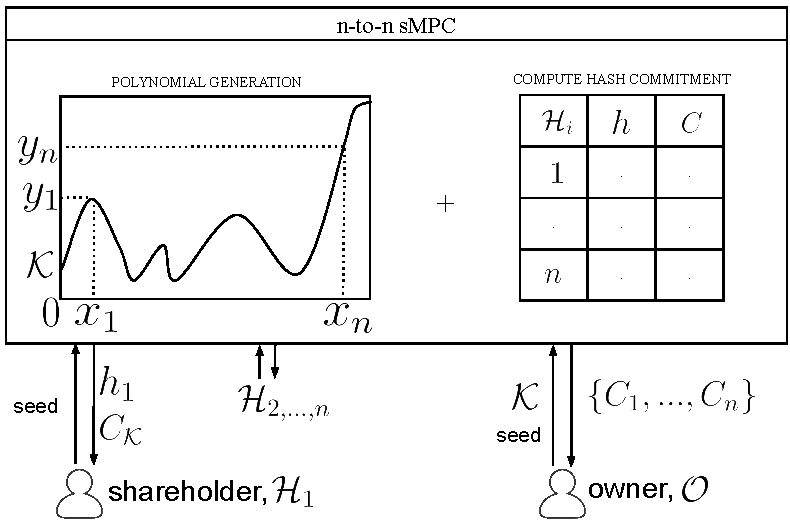
\includegraphics[width=0.9\columnwidth]{fig/mpc_rev_1.pdf}
	\caption{Single-phase sMPC protocol jointly executed by all the participants}
	\label{fig:mpc1}
\end{figure}

Nevertheless, \shortname is a game played by rational adversaries, so the participants could look at sMPC techniques from another perspective.
Actually, the malicious coalition of shareholders, \coalition, could devise a strategy that permits to recover and sell \secret without incurring in economic penalties. 
Such a strategy would have been successful if it did not allow anyone to satisfy the smart contract commitments.
In our setting, it means to recover \secret without exposing \key, and therefore preventing anyone to invoke the \texttt{WhistleblowSecret} function.
As a matter of fact, the malicious coalition can instantiate an offensive sMPC that receives as input at least $k$-of-$n$ shares plus the ciphertext, \ciphertext.
Then, it performs internally both the reconstruction of \key and the extraction of the secret by \unwrap.
Finally, it outputs to all the attackers only \secret. 

To prevent the execution of this attack it is sufficient to select a cryptosystem \cipvocabulary such that there is no sMPC protocol that permits to execute \dec by producing \secret as the only output.
We identified two possible alternatives to satisfy the previous requirement.

\begin{enumerate}
	\item Use a cryptosystem that ensure that the exposure of \secret implies exposing also the \key (by the key it is possible to perform the whistleblow protocol).
	\item Use a cryptosystem whose execution is not compatible with sMPC protocols.
\end{enumerate}

We can satisfy the first condition by selecting $ \mathcal{\cip}=$$ \text{ }\onetimepad$. 
It is easy to prove that given two among $\{ \ciphertext , \secret , \key \}$ the third is implied. 
Thus, each member of the malicious coalition could invoke the \texttt{WhistleblowSecret} function after obtaining \secret. 
The drawback of using \onetimepad, is that $|\secret| = |\key|$ by construction. 
This limitation can be overcome by selecting a cryptosystem that satisfies the second condition; however devising a strategy to construct such a cryptosystem goes beyond the scope of this chapter.

\df{possiamo usare la cosa seguente in qualche modo?}
The consideration that stem from the use of adversarial sMPC are interesting, as this kind of attacks (i.e., programming the logic of a protocol inside a sMPC to bypass hashlocks) are applicable to all protocols that involve rewards, penalties and are played by rational adversaries.

\subsection{DOS Attacks and Deadlocks prevention}
%In order to meet the functionalities presented in sections~\ref{sect:model} and ~\ref{sect:constraints}, we introduced some additional features.  
%As mentioned in Subsection~\ref{sect:mal_sha}, we allowed the owner to set a maximum disclosure time deadline, or rather a time instant to which the registration of less than $k$ shares determines the failure of \shortname. The extra remuneration, $\delta$, for the fastest $k$ registering shareholders has also been integrated. 

A denial of service attack could be performed by some users who take part in many \shortname protocol instances refusing to deposit the bids, to commit or to correctly execute the sMPC. 
To mitigate these kind of disruptions it is possible to introduce a reputation system, so that the owner can select parties that are willing to co-operate. 
Obviously this would be an ideal choice that could benefit also other parts of our model. However, as the introduction of a reputation model is not always possible, we decided to model the smart contract \texttt{PRE\textunderscore CONSIDERED} state. 
Specifically, all the participants (including the owner) are required to pay an additional small service pawn that will be returned only if the smart contract will reach the \texttt{LOCKED} state. 
It has been proved that introducing a small fee to access a service can prevent many DOS attacks~\cite{ddos-payments,ddos-survey}. 
Furthermore, some malfunctions or network errors may imply the time thresholds set by the owner not being met.
The deadlock to which the protocol would lead to can be solved by the presence of the final state \texttt{EXPIRED}. 
In that event, all the participants are allowed to withdraw their funds locked in the contract.  